\documentclass{article}
\usepackage[utf8]{inputenc}
\usepackage{graphicx}
\usepackage{xcolor}
\definecolor{mydarkgray}{RGB}{55, 55, 55}
\definecolor{mydarkviolet}{RGB}{102, 0, 153}
\usepackage[hidelinks, colorlinks=true, linkcolor=mydarkviolet, urlcolor=mydarkviolet, citecolor=cyan]{hyperref}
\usepackage{listings}
\usepackage{ragged2e}  
\usepackage{float}
\usepackage{url} 
\usepackage{animate}

\title{\Huge \textbf{Proyecto Final: Sistema de Observación Meteorológica}}
\author{
  Jorge Domínguez González (\href{mailto:alu0101330600@ull.edu.es}{alu0101330600@ull.edu.es}) \and
  Adnan Hawari Capa (\href{mailto:Alu0100417012@ull.edu.es}{Alu0100417012@ull.edu.es}) \and
  Paula Regalado De León (\href{mailto:Alu0101330174@ull.edu.es}{Alu0101330174@ull.edu.es})
}
\date{\today}

\begin{document}
\maketitle

\tableofcontents
\listoffigures
\newpage

\section{Introducción}
\subsection{Práctica anterior}
En la anterior práctica se presenta una implementación de un sistema de observación meteorológica en Java. Este sistema utiliza el patrón de diseño Observador para recibir actualizaciones de las condiciones meteorológicas de diversas ciudades a través de la API de WeatherStack. WeatherStack es un servicio de API de pronóstico del tiempo que proporciona información actualizada sobre condiciones meteorológicas actuales, incluyendo temperatura, velocidad del viento, humedad, presión atmosférica y más.

\subsection{Objetivo de la Práctica}
El objetivo de la práctica es implementar un historial de los distintos datos recibidos, es decir, desarrollar una aplicación de visualización de datos meteorológicos utilizando Java y el framework JFreeChart. La aplicación permite seleccionar una ciudad y visualizar datos meteorológicos como temperatura, probabilidad de precipitación, velocidad del viento, presión atmosférica y cobertura de nubes. Además, el usuario puede elegir entre dos tipos de gráficos: líneas y barras.

\section{Estructura del Directorio}
En la figura \ref{fig:estructura-proyecto} podemos observar la estructura de nuestro proyecto.

\begin{figure}[H]
  \centering
  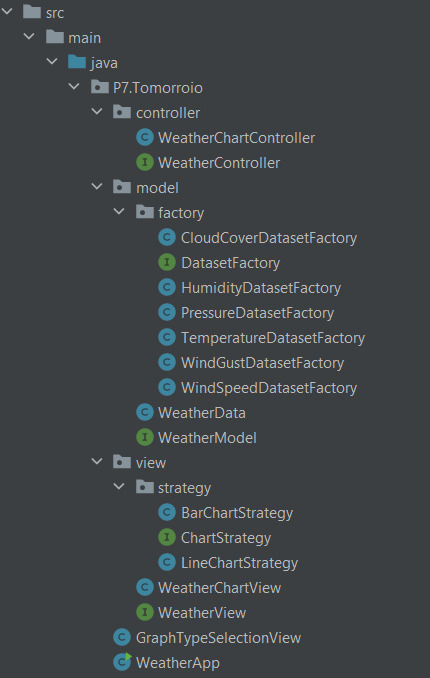
\includegraphics[width=0.8\textwidth]{images/image6.png}
  \caption{Estructura del directorio del proyecto.}
  \label{fig:estructura-proyecto}
\end{figure}

\section{Estructura del Código}
\subsection{Clase WeatherApp}
Este archivo es el punto de entrada principal de la aplicación. Utiliza Swing para crear la interfaz de usuario y permite al usuario seleccionar la ciudad y el tipo de gráfico. Inicia la aplicación mediante la creación de instancias de las vistas y controladores necesarios.

\subsection{Clase WeatherView}
Interfaz que define el método updateChart para actualizar los gráficos.

\subsubsection{Clase WeatherChartView}
Implementa la interfaz WeatherView. Crea y muestra una ventana que contiene gráficos JFreeChart. Utiliza estrategias de gráficos (ChartStrategy) para determinar el tipo de gráfico (líneas o barras). Proporciona métodos para agregar paneles de gráficos y actualizar los datos de los gráficos.

\subsection{Clase GraphTypeSelectionView}
Crea una ventana Swing para que el usuario seleccione el tipo de gráfico y la ciudad.

\subsection{Clase ChartStrategy}
Interfaz que define el contrato para las estrategias de creación de gráficos.

\subsubsection{Clase LineChartStrategy}
Implementa la interfaz ChartStrategy. Proporciona una estrategia específica para crear un gráfico de líneas utilizando JFreeChart.

\subsubsection{Clase BarChartStrategy}
Implementa la interfaz ChartStrategy. Proporciona una estrategia específica para crear un gráfico de barras utilizando JFreeChart.

\subsection{Clase WeatherData}
Implementa la interfaz WeatherModel. Obtiene datos meteorológicos de la API de Tomorrow.io utilizando la biblioteca Unirest. Convierte y almacena los datos en series temporales (XYSeries) para su uso en los gráficos.

\subsection{Clase DatasetFactory}
La interfaz `DatasetFactory` define el contrato para las fábricas de conjuntos de datos meteorológicos. A través de esta interfaz, especificamos los métodos necesarios que las factorías concretas deben implementar para la creación de conjuntos de datos.

\subsubsection{Clase XDatasetFactory}
La clase `XDatasetFactory` implementa la interfaz `DatasetFactory`. Es una factoría abstracta que proporciona métodos específicos para crear conjuntos de datos basados en el tipo de dato meteorológico. Esta factoría concreta se especializa en la creación de conjuntos de datos de tipo `XYSeriesCollection`.

\subsubsection{Clase TemperatureDatasetFactory}
La clase `TemperatureDatasetFactory` es una implementación concreta de `DatasetFactory` especializada en la creación de conjuntos de datos para la temperatura. Hereda de `XDatasetFactory` y proporciona la implementación específica para crear conjuntos de datos de temperatura.

\subsubsection{Clase HumedityDatasetFactory}
La clase `HumedityDatasetFactory` es otra implementación concreta de `DatasetFactory`. Al igual que las otras factorías, hereda de `XDatasetFactory` y se centra en la creación de conjuntos de datos para la probabilidad de Humedad.

\subsubsection{Clase WindSpeedDatasetFactory}
La clase `WindSpeedDatasetFactory` implementa `DatasetFactory` y se especializa en la creación de conjuntos de datos para la velocidad del viento. También hereda de `XDatasetFactory` y proporciona la implementación necesaria para este tipo de dato meteorológico.

\subsubsection{Clase PressureDatasetFactory}
La clase `PressureDatasetFactory` es una implementación concreta para la creación de conjuntos de datos relacionados con la presión atmosférica. Al igual que las otras factorías, hereda de `XDatasetFactory` y ofrece la implementación específica para datos de presión.

\subsubsection{Clase CloudCoverDatasetFactory}
La clase `CloudCoverDatasetFactory` implementa `DatasetFactory` y se encarga de la creación de conjuntos de datos para la cobertura de nubes. Hereda de `XDatasetFactory` y proporciona la implementación necesaria para este tipo de dato meteorológico.

Estas clases concretas de factorías implementan métodos específicos para la creación de conjuntos de datos relacionados con sus respectivos tipos de datos meteorológicos. Al emplear el patrón Abstract Factory, logramos una estructura modular que facilita la extensión del sistema al agregar nuevos tipos de datos meteorológicos en el futuro.

\subsection{Clase WeatherChartController}
Implementa la interfaz WeatherController. Coordina la actualización de los gráficos mediante la creación de instancias de las fábricas de conjuntos de datos y la actualización de la vista. El proyecto utiliza de manera efectiva patrones de diseño como el patrón Estrategia para los diferentes tipos de gráficos y el patrón Fábrica para la creación de conjuntos de datos meteorológicos.

\section{Diagrama UML y Patrones}
En esta práctica usamos varios patrones que hemos visto a lo largo de la asignatura, como puede ser el patrón estrategia, el abstract factory y el modelo de vista controlador que iremos señalando en el siguiente apartado:

\subsection{Patrón Estrategia}
El patrón de diseño Estrategia se ha utilizado para la elección de gráficos en la aplicación debido a su capacidad para encapsular algoritmos intercambiables y permitir que el cliente seleccione dinámicamente uno de ellos. Como podemos observar en la image 2, el usuario puede seleccionar la gráfica de líneas o la gráfica de barras.

\begin{figure}[H]
  \centering
  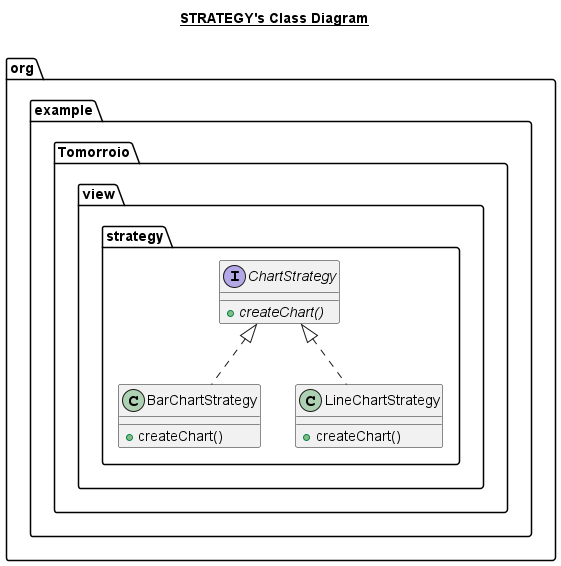
\includegraphics[width=0.8\textwidth]{images/image2.png}
  \label{fig:image2}
\end{figure}

\subsection{Patrón Abstract Factory}
El patrón de diseño Abstract Factory se ha utilizado como se puede observar en la figura \ref{fig:image7} para crear de forma dinámica los diferentes tipos de datos de forma ordenada y flexible.

\begin{figure}[H]
  \centering
  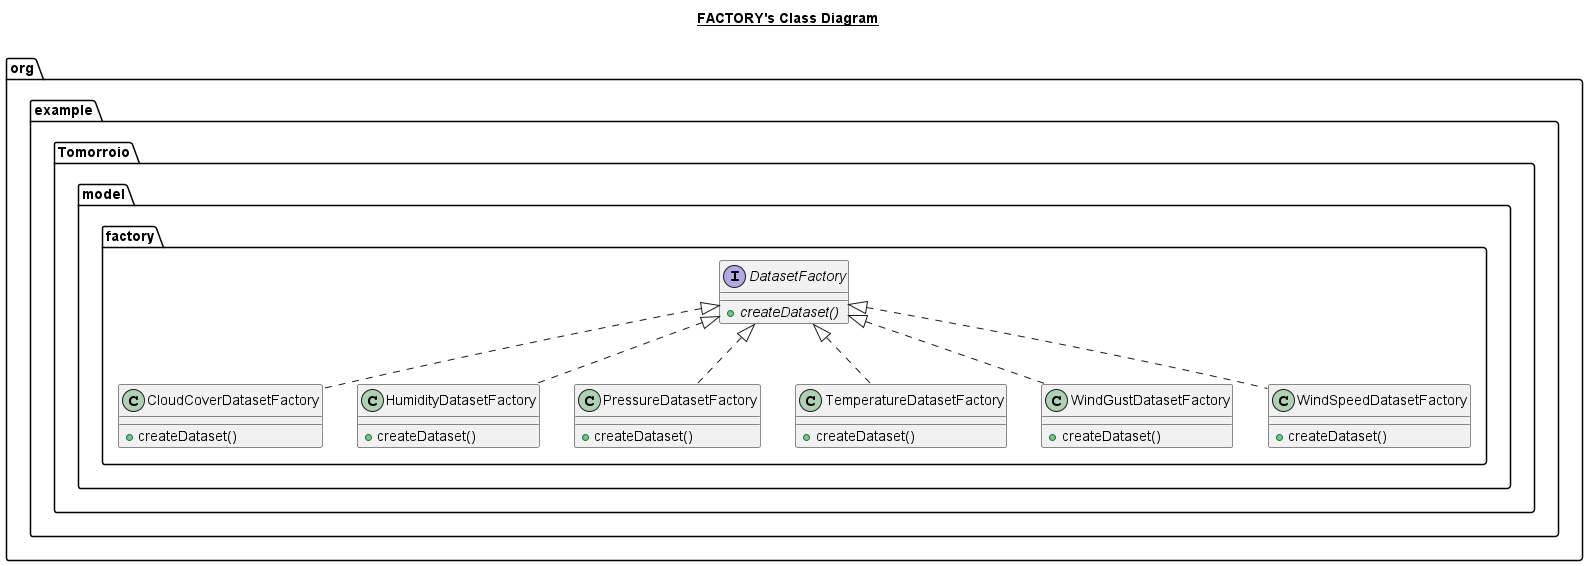
\includegraphics[width=1.1\textwidth]{images/image7.png}
  \label{fig:image7}
\end{figure}

\subsection{Patrón Modelo Vista Controlador}
El patrón de diseño Modelo Vista Controlador se ha utilizado para separar por capas los diferentes modelos de la aplicación.

\begin{figure}[H]
  \centering
  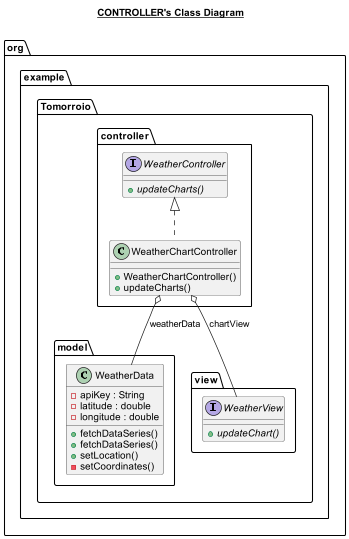
\includegraphics[width=1.1\textwidth]{images/image3.png}
  \label{fig:image3}
\end{figure}

\section{Pasos del Flujo del Programa}
El programa sigue estos pasos:

\begin{enumerate}
  \item El usuario interactúa con la interfaz gráfica, seleccionando el tipo de gráfico y la ciudad en GraphTypeSelectionView.
  \item GraphTypeSelectionView envía eventos al controlador (WeatherChartController).
  \item WeatherChartController utiliza la información proporcionada por el usuario para obtener datos meteorológicos actualizados de WeatherData.
  \item Se crean conjuntos de datos utilizando fábricas (DatasetFactory) para diferentes tipos de datos meteorológicos.
  \item WeatherChartController actualiza la vista (WeatherChartView) con los nuevos conjuntos de datos.
\end{enumerate}

\section{Interfaz Gráfica para el Usuario}
La interfaz gráfica incluye un formulario para que el usuario seleccione el tipo de gráficos como vemos en la figura \ref{fig:seleccion_ciudad}  y la ciudad de interés como vemos en la figura \ref{fig:seleccion_ciudad2}  y una pantalla para mostrar el historial de temperatura, precipitación, viento, presión y nubes, en la figura \ref{fig:seleccion_ciudad3} podemos ver un ejemplo para Tokio representado en líneas y en la figura \ref{fig:seleccion_ciudad4} para Tokio representado en barras, donde se actualiza en tiempo real la información.

\begin{figure}[H]
    \centering
    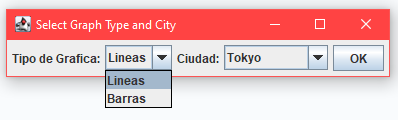
\includegraphics[width=0.5\textwidth]{images/image5.png}
    \caption{Interfaz gráfica para el usuario.}
    \label{fig:seleccion_ciudad}
\end{figure}

\begin{figure}[H]
    \centering
    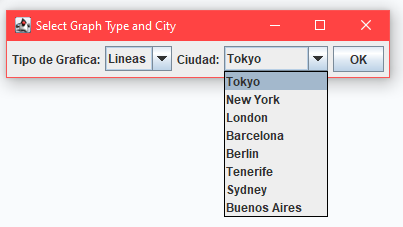
\includegraphics[width=0.7\textwidth]{images/image9.png}
    \caption{ Interfaz gráfica para el usuario.}
    \label{fig:seleccion_ciudad2}
\end{figure}

\begin{figure}[H]
  \centering
  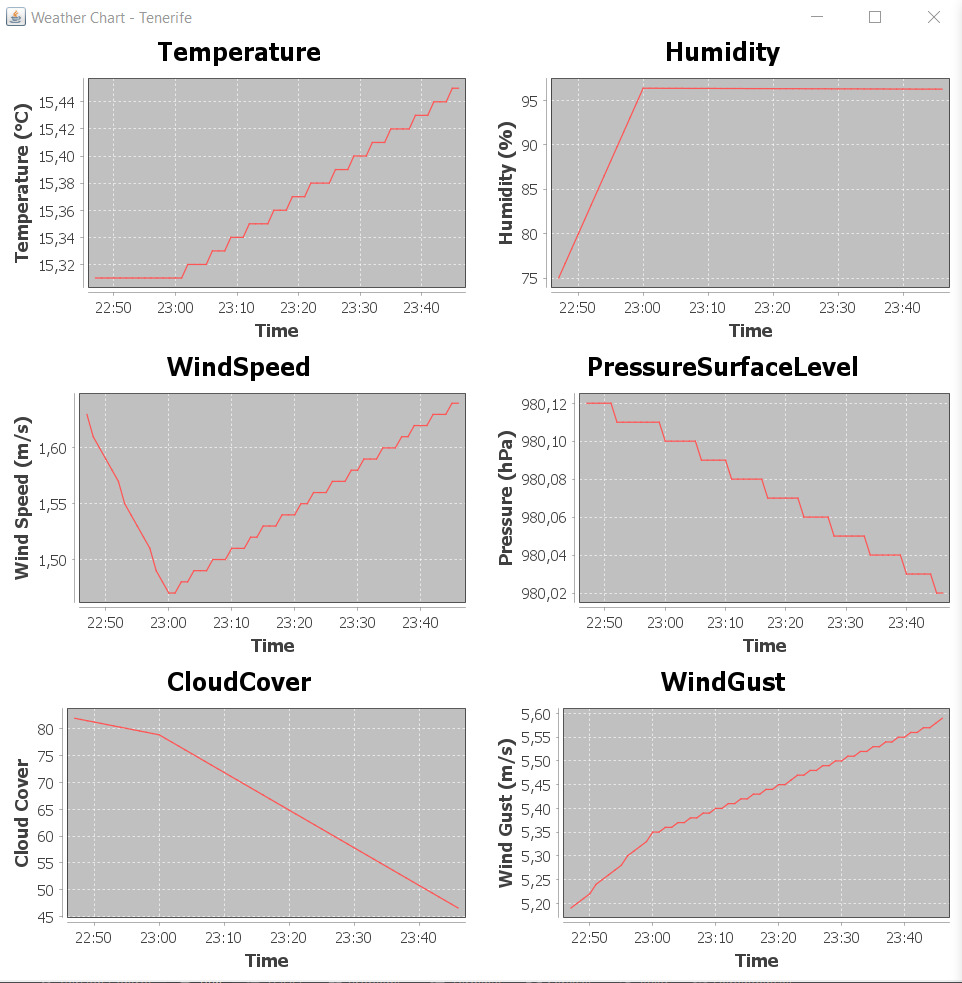
\includegraphics[width=0.7\textwidth]{images/image4.png}
  \caption{Interfaz gráfica para el usuario.}
  \label{fig:seleccion_ciudad3}
\end{figure}

\begin{figure}[H]
  \centering
  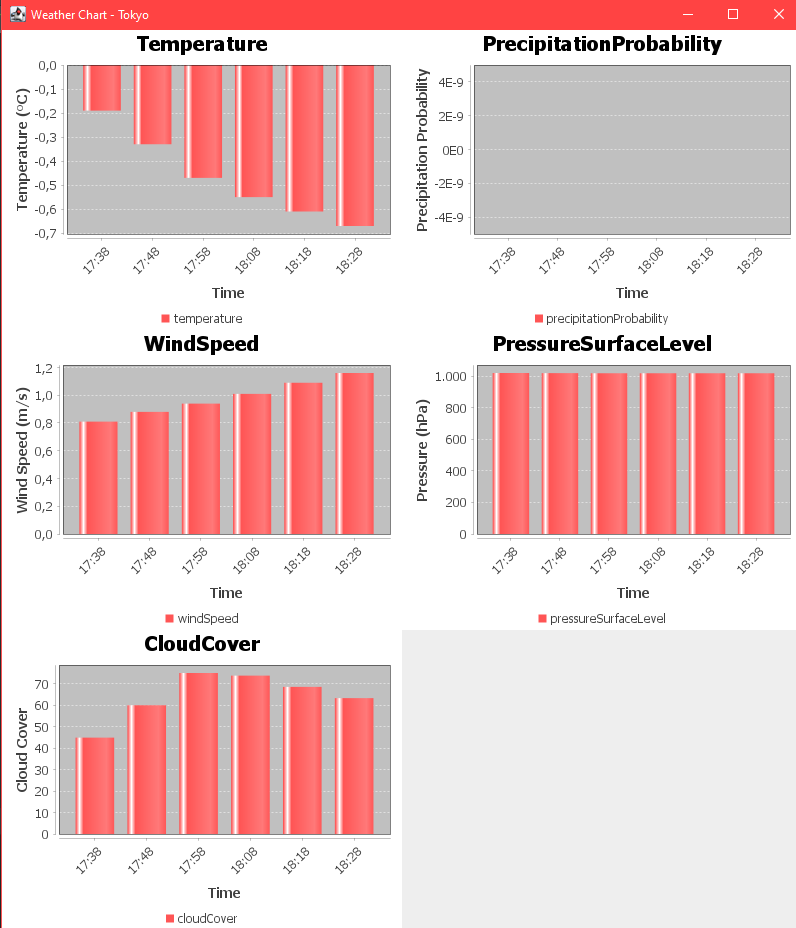
\includegraphics[width=0.7\textwidth]{images/image10.png}
  \caption{Interfaz gráfica para el usuario.}
  \label{fig:seleccion_ciudad4}
\end{figure}

\section{Diagrama UML}
El diagrama UML del proyecto se muestra en la Figura \ref{fig:uml}.

\begin{figure}[H]
    \centering
    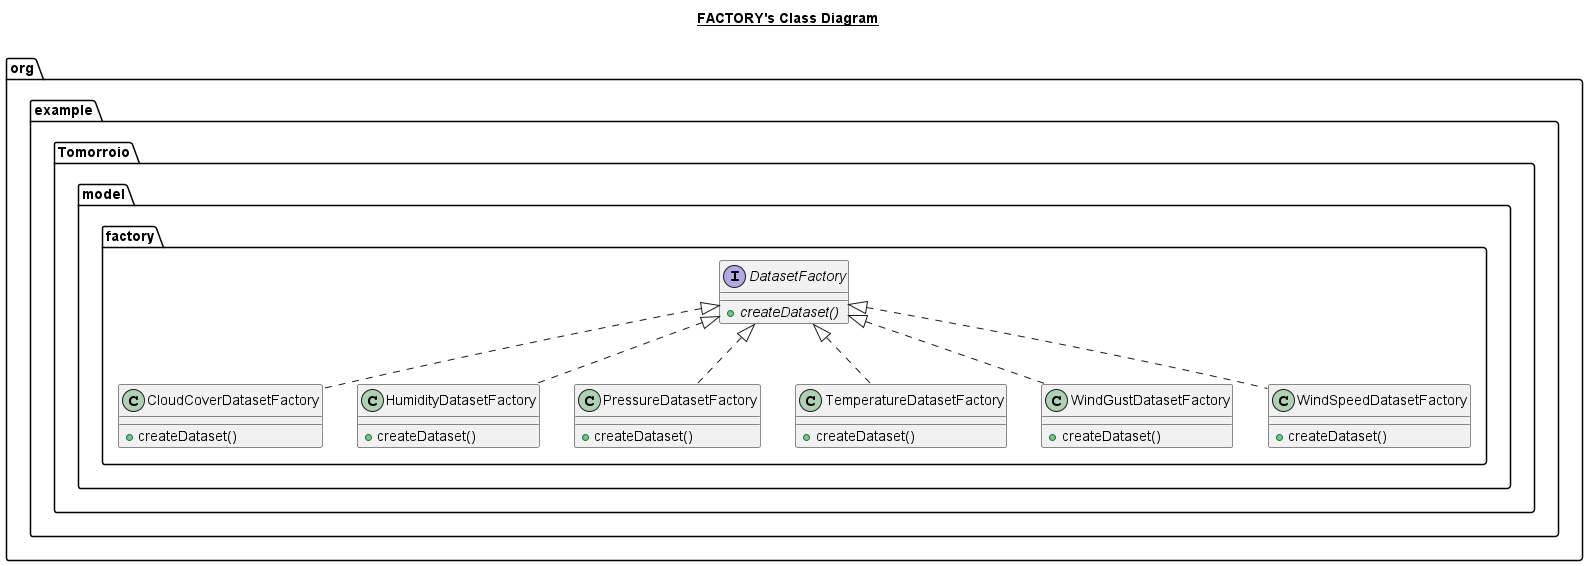
\includegraphics[width=1.0\textwidth]{images/image7.png}
    \caption{Diagrama UML del proyecto.}
    \label{fig:uml}
\end{figure}

\section{Errores y Desafíos Encontrados}
Durante el desarrollo de este proyecto, nos enfrentamos a varios desafíos que requirieron soluciones creativas y resolución de problemas. A continuación, destacamos algunos de los errores y desafíos más significativos y cómo abordamos cada uno:

\subsection{Conexión con la API de Tomorrow.io}
Uno de los desafíos iniciales fue establecer una conexión efectiva con la API de Tomorrow.io para obtener datos meteorológicos en tiempo real. En algunos casos, experimentamos problemas de tiempo de espera y errores de conexión. Para superar esto, implementamos un manejo robusto de errores y optimizamos nuestras solicitudes para mejorar la eficiencia.

\subsection{Sincronización de Datos en Tiempo Real}
La sincronización de datos en tiempo real para proporcionar actualizaciones constantes en la interfaz gráfica fue un desafío importante. Implementamos un mecanismo de actualización basado en eventos para garantizar que los gráficos reflejaran con precisión los datos meteorológicos más recientes. Esto implicó coordinar eficientemente la obtención de datos, su procesamiento y la actualización de la interfaz de usuario.

\subsection{Manejo de Excepciones}
En el proceso de desarrollo, identificamos la necesidad de un manejo exhaustivo de excepciones para garantizar la estabilidad y la usabilidad de la aplicación. Implementamos una estrategia sólida de manejo de excepciones para notificar al usuario sobre posibles problemas y evitar fallos inesperados.

Estos desafíos contribuyeron significativamente a nuestro aprendizaje y resiliencia durante el desarrollo del proyecto. La capacidad para superar estos obstáculos mejoró nuestras habilidades de resolución de problemas y fortaleció la calidad general del sistema.

\section{Estimación de Plazo}
\begin{table}[H]
  \centering
  \caption{Estimación de Plazo}
  \begin{tabular}{|c|c|c|}
    \hline
    \textbf{Tarea} & \textbf{Tiempo Estimado} & \textbf{Tiempo Real} \\
    \hline
    Elegir propuesta & 30 minutos & 15 minutos \\
    Implementar JFreeChart & 1 hora & 1 hora y media \\
    Obtener datos historial & 30 minutos & 45 minutos \\
    Implementar patrones & 1 hora & 45 minutos \\
    Implementar interfaces & 2 horas & 2 horas y media \\
    Pruebas y depuración & 2 horas & 3 horas \\
    Documentación & 1 hora & 1 hora y media \\
    Implementación Github & 1 hora y media & 1 hora y media \\
    \hline
  \end{tabular}
  \label{Estimación de Plazo}
\end{table}

\section{Conclusiones}
En conclusión, el uso de patrones de diseño ha simplificado el diseño y la implementación de la aplicación. Ha proporcionado una estructura modular y extensible, facilitando la incorporación de nuevas funcionalidades en algún futuro. Además de utilizar diferentes herramientas, como el JFreeChart, para realizar un proyecto bastante práctico y elaborado.

\section{Bibliografía}
\begin{thebibliography}{99}
    \bibitem Tomorrow.io API: \url{https://www.tomorrow.io/}
    \bibitem Unirest: \url{http://kong.github.io/unirest-java/}
    \bibitem JFreeChart: \url{https://www.jfree.org/jfreechart/}
    \bibitem JFreeChart Developer Guide: \url{https://www.jfree.org/jfreechart/api/javadoc/org/jfree/chart/JFreeChart.html}
    \bibitem JFreeChart Tutorial: \url{https://www.tutorialspoint.com/jfreechart/index.htm}
    \bibitem JFreeChart Tutorial: \url{https://www.tutorialspoint.com/jfreechart/jfreechart_quick_guide.htm}
    \bibitem JFreeChart Tutorial: \url{https://www.tutorialspoint.com/jfreechart/jfreechart_overview.htm}
    \bibitem JFreeChart Tutorial: \url{https://www.tutorialspoint.com/jfreechart/jfreechart_xy_chart.htm}
    \bibitem JFreeChart Tutorial: \url{https://www.tutorialspoint.com/jfreechart/jfreechart_bar_chart.htm}
    \bibitem JFreeChart Tutorial: \url{https://www.tutorialspoint.com/jfreechart/jfreechart_line_chart.htm}
    \bibitem JFreeChart Tutorial: \url{https://www.tutorialspoint.com/jfreechart/jfreechart_pie_chart.htm}
    \bibitem WeatherStack API: \url{https://weatherstack.com/}
    \bibitem JFreeChart: \url{https://sourceforge.net/projects/jfreechart/}
    \bibitem Observador (patrón de diseño): \url{https://es.wikipedia.org/wiki/Observer_(patr%C3%B3n_de_dise%C3%B1o)}
    \bibitem Estrategia (patrón de diseño): \url{https://es.wikipedia.org/wiki/Estrategia_(patr%C3%B3n_de_dise%C3%B1o)}
    \bibitem Fábrica abstracta: \url{https://es.wikipedia.org/wiki/F%C3%A1brica_abstracta}
    \bibitem Modelo–vista–controlador: \url{https://es.wikipedia.org/wiki/Modelo%E2%80%93vista%E2%80%93controlador}
    \bibitem Patrones de diseño: \url{https://es.wikipedia.org/wiki/Patr%C3%B3n_de_dise%C3%B1o_de_software}
    \bibitem Patrones de diseño: \url{https://www.tutorialspoint.com/design_pattern/index.htm}
    \bibitem Patrones de diseño: \url{https://www.geeksforgeeks.org/software-design-patterns/}
    \bibitem Patrones de diseño: \url{https://www.journaldev.com/1827/java-design-patterns-example-tutorial}
    \bibitem Patrones de diseño: \url{https://www.javatpoint.com/design-patterns-in-java}
\end{thebibliography}

\end{document}